\section{The Serial Safety Net}
Das Serial Safety Net baut auf bestehenden Multiversion-Concurrency-Control-Verfahren auf.
In einem System, welches Multiversion-Concurrency-Control(MVCC) verwendet, bestehen alle Datenbankelemente aus einer Sequenz von Versionen, wobei Schreiboperationen jeweils eine Version anlegen und Leseoperationen eine Version zurückgeben.

Für solche MVCC-Verfahren sichert das Serial Safety Net einen kreisfreien Abhängigkeitsgraphen, wodurch die Serialisierbarkeit des Transaktionsplans gewährleistet wird.
Der Abhängigkeitsgraph stellt dabei eine Übersicht über die Abhängigkeit zwischen den Transaktionen eines Plans dar, wobei die Knoten des Graphen die committeten Transaktionen und die Kanten die Abhängigkeiten zwischen diesen darstellen.
Ein Graph ohne Zyklen garantiert dabei immer, dass ein äquivalenter serieller Plan zu den ausgeführten Transaktionen existiert, welcher zum selben Ergebnis geführt hätte.

\begin{Definition}
	Die Abhängigkeit $T\leftarrow U$ zwischen den Transaktionen $T$ und $U$ besagt, dass $U$ von $T$ abhängig ist und somit $T$ als direkter Vorgänger und $U$ als direkter Nachfolger bezeichnet wird.
\end{Definition}

Es gibt zwei verschiedene Arten von Abhängigkeiten zwischen Transaktionen:
\begin{itemize}
	\item $T_i\xleftarrow{w:x}T$ - \textbf{Lese-/Schreibabhängigkeit}: $T$ greift auf eine Version zu, welche $T_i$ erstellt hat, weshalb $T$ nach $T_i$ serialisiert werden muss
	\item $T\xleftarrow{r:w}T_j$ - \textbf{Anti-Abhängigkeit}: $T$ liest eine Version, die $T_j$ überschrieben hat, weshalb $T$ vor $T_j$ serialisiert werden muss
\end{itemize}

Eine zentrale Rolle bei der Umsetzung des Serial Safety Nets spielt die Untersuchung der Abhängigkeiten von Transaktionen in Verbindung mit der Commit-Reihenfolge.
Dazu lassen sich zwei verschiedene Typen von Abhängigkeiten wie folgt definieren.

\begin{Definition}
	Bei einer \textcolor{my-green}{Back-Edge} $T\xleftarrow{b} U$ committet der Nachfolger $U$ zuerst.
\end{Definition}

\begin{Definition}
	Bei einer \textcolor{my-blue}{Forward-Edge} $T\xleftarrow{f} U$ committet der Vorgänger $T$ zuerst.
\end{Definition}

\begin{Definition}
	Eine reflexive, transitive \textcolor{my-green}{Back-Edge} $T\xleftarrow{b*} U$ bezeichnet eine Verbindung, bei der $T$ von $U$ ausschließlich über Back-Edges erreichbar ist.
\end{Definition}

\begin{figure}
	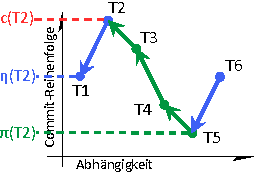
\includegraphics{img/Figure_2_1.pdf}
	\caption{Veranschaulichung von \textcolor{my-green}{Back}- und \textcolor{my-blue}{Forward-Edges} sowie den Zeitstempeln von Transaktion $T2$}
	\label{fig:back_forward}
\end{figure}

Zum besseren Verständnis sind die genannten Begriffe in Abbildung \ref{fig:back_forward} veranschaulicht worden.
Die abgebildeten Back-Edges ergeben zusammen eine reflexive, transitive Back-Edge von Transaktion $T2$ zu $T5$.

Die Umsetzung des Serial Safety Nets erfordert das Erfassen der folgenden drei Zeitstempel zu jeder Transaktion, welche es später erlauben einen Abhängigkeitszyklus zu erkennen.
Die vorgestellten Zeitstempel sind ebenfalls in Abbildung \ref{fig:back_forward} für die Transaktion $T2$ eingezeichnet.

\begin{Definition}
	\textcolor{my-red}{$c(T)$} bezeichnet die Commit-Zeit der Transaktion $T$
\end{Definition}

\begin{Definition}
	\textcolor{my-green}{$\pi (T)$} bezeichnet die Commit-Zeit des ältesten Nachfolgers, der durch Back-Edges erreichbar ist:\\		
	$\pi (T)=\min (c(U):T\xleftarrow{b*}U)=\min (\{\pi (U):T\xleftarrow{b}U\}\cup \{c(T)\})$
\end{Definition}

\begin{Definition}
	\textcolor{my-blue}{$\eta (T)$} bezeichnet die Commit-Zeit des zuletzt committeten Vorgängers von $T$:\\
	$\eta (T) = \max (\{c(U):U\xleftarrow{f} T\}\cup \{-\infty \})$
\end{Definition}

Mithilfe dieser Zeitstempel lässt sich nun für jede Transaktion $T$ ein sogenanntes Ausschlussfenster definieren, welches garantiert, dass ein Vorgänger von $T$ nicht gleichzeitig ein Nachfolger sein kann, was auf einen Abhängigkeitskreis hinweisen würde.
Eine Verletzung dieses Ausschlussfensters durch eine Abhängigkeit $U\leftarrow T$ lässt sich feststellen, wenn ein Vorgänger $U$ gefunden wird, sodass die folgende Ungleichung erfüllt ist.

\begin{equation}
	\textcolor{my-green}{\pi (T)} \leq \textcolor{my-yellow}{c(U)} \leq \textcolor{my-red}{c(T)}
	\label{eq:ausschlussfenster_lang}
\end{equation}

Gibt es für die Transaktion $T$ also einen Vorgänger $U$, welcher nach dem ältesten Nachfolger von $T$, nämlich \textcolor{my-green}{$\pi (T)$}, committet wurde, dann kann nicht sichergestellt werden, dass $U$ nicht auch ein Nachfolger von $T$ ist.
Dies liegt daran, dass die Transaktion nichts über die Nachfolger von \textcolor{my-green}{$\pi (T)$} weiß und es somit möglich wäre, dass $U$ einer dieser Nachfolger ist, was damit einen Abhängigkeitszyklus bedeuten würde.

In dem Beispiel aus Abbildung \ref{fig:back_forward} ist erkennbar, dass für die Transaktion $T2$ eine solche Verletzung des Ausschlussfensters vorliegt, da die Transaktion $T1$, welche ein Vorgänger von $T2$ ist, zwischen \textcolor{my-red}{$c(T2)$} und \textcolor{my-green}{$\pi (T2)$} committet wurde.
Dies wird außerdem klar dadurch, dass die Transaktion $T6$ in diesem Beispiel ebenfalls die Transaktion $T1$ sein könnte, wovon $T2$ nicht direkt etwas wüsste.
Damit wäre der Abhängigkeitszyklus entstanden und der Plan nicht serialisierbar.

Um die Umsetzung des Serial Safety Nets einfacher und performanter zu gestalten, lässt sich die Ungleichung \ref{eq:ausschlussfenster_lang} noch weiter vereinfachen.
Zum einen müssen nur Vorgänger betrachtet werden, welche vor $T$ committet wurden, da ansonsten der zweite Teil der Ungleichung automatisch nicht erfüllt wäre.
Dies eröffnet die Freiheit das Überprüfen des Ausschlussfensters erst zum Commit-Zeitpunkt der betrachteten Transaktion zu überprüfen.

Außerdem wird nur der Vorgänger von $T$ betrachtet, dessen Commit-Zeitpunkt am spätesten ist, da dieser maßgebend für das Erfüllen des ersten Teils der Ungleichung ist.
Wie vorher beschrieben wird die Commit-Zeit des zuletzt committeten Vorgängers von $T$ mit \textcolor{my-blue}{$\eta (T)$} bezeichnet, wodurch die Ungleichung \ref{eq:ausschlussfenster_lang} folgendermaßen vereinfacht wird.

\begin{equation}
	\textcolor{my-green}{\pi (T)} \leq \textcolor{my-blue}{\eta (T)}
	\label{eq:ausschlussfenster_kurz}
\end{equation}

Wird diese Bedingung auf das in Abbildung \ref{fig:back_forward} beschriebene Beispiel angewendet, wird deutlich, dass die Ungleichung für Transaktion $T2$ erfüllt ist und somit eine Verletzung des Ausschlussfensters erkannt wird.
